% p10-06 引入：正方形 ABCD 边长 8, E 在 BC 上 BE=3 EC=5; 把 △ABE 绕 A 逆时针 90° → △ADE'
% A(0,0), B(8,0), C(8,8), D(0,8)；E=(8,3)
% 逆时针 90° 绕 A: (x,y)→(-y,x)；B(8,0)→(0,8)=D ✓；E(8,3)→(-3,8)
\documentclass[tikz,border=4pt]{standalone}
\usepackage{ctex}
\usepackage{amsmath}
\usetikzlibrary{calc, arrows.meta}
\begin{document}
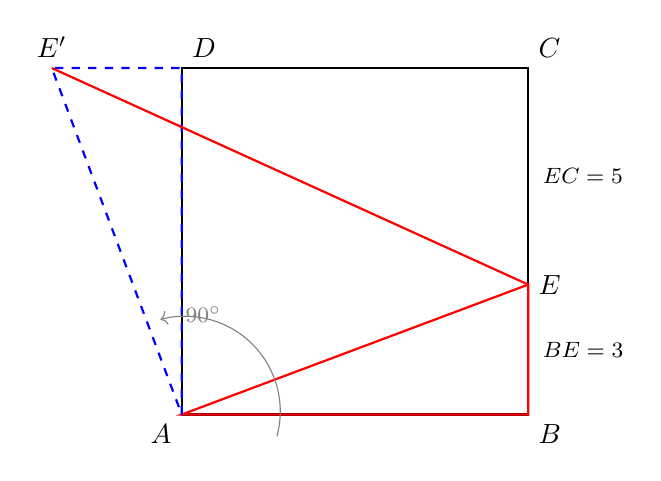
\begin{tikzpicture}[scale=0.55, thick]
  \coordinate (A) at (0,0);
  \coordinate (B) at (8,0);
  \coordinate (C) at (8,8);
  \coordinate (D) at (0,8);
  \coordinate (E) at (8,3);
  \coordinate (Ep) at (-3,8);

  \draw (A)--(B)--(C)--(D)--cycle;

  % △ABE 原（红实线）
  \draw[red, thick] (A)--(B)--(E)--cycle;
  % △ADE' 旋转后（蓝虚线）
  \draw[blue, dashed, thick] (A)--(D)--(Ep)--cycle;
  % △AEE'
  \draw[red, thick] (E)--(Ep);

  % 旋转弧示意
  \draw[->, gray, thin] (2.2, -0.5) arc[start angle=-15, end angle=105, radius=2.2];
  \node[gray, font=\footnotesize] at (0.5, 2.3) {$90^\circ$};

  \node[below left]  at (A) {$A$};
  \node[below right] at (B) {$B$};
  \node[above right] at (C) {$C$};
  \node[above right] at (D) {$D$};
  \node[right] at (E) {$E$};
  \node[above] at (Ep) {$E'$};

  \node[font=\footnotesize, right] at (8.1, 1.5) {$BE=3$};
  \node[font=\footnotesize, right] at (8.1, 5.5) {$EC=5$};
\end{tikzpicture}
\end{document}
